\documentclass[9pt,twocolumn,twoside,lineno]{style}

\articletype{NEI} % article type

\title{Aoki in Ménard (2000, capítulo 3): \textit{Institutional evolution as punctuated equilibria}}
\date{1º Semestre de 2020}

\author[$\ddagger$]{Gabriel Petrini}

\affil[$\ddagger$]{Doutorando no instituto de Economia da Unicamp}

\keywords{Keyword \\ Keyword2 \\ Keyword3 \\ ...}

\runningtitle{Fichamento} % For use in the footer 

%% For the footnote.
\runningauthor{Petrini}

\begin{abstract}
\end{abstract}

\begin{document}

\maketitle
\articletypemark
\marginmark
\thispagestyle{firststyle}

% Please add here a significance statement to explain the relevance of your work
%\afterpage{
%	\begin{sigstatement}
%		\sffamily
%		\mdfdefinestyle{stylesigstyle}{linewidth=0.7pt,
%			backgroundcolor=styleblueback,linecolor=stylebluetext,
%			fontcolor=stylebluetext,innertopmargin=6pt,innerrightmargin=6pt,
%			innerbottommargin=6pt,innerleftmargin=6pt}
%		{%	
%			\begin{mdframed}[style=stylesigstyle]%
%				\section*{5 Seconds Synthesis}%
%				\lipsum[1-3]
%		\end{mdframed}}
%\end{sigstatement}
%}

% If your first paragraph (i.e. with the \dropcap) contains a list environment (quote, quotation, theorem, definition, enumerate, itemize...), the line after the list may have some extra indentation. If this is the case, add \parshape=0 to the end of the list environment.


\afterpage{
	\begin{sigstatement}
		\sffamily
		\mdfdefinestyle{stylesigstyle}{linewidth=0.7pt,backgroundcolor=styleblueback,linecolor=stylebluetext,fontcolor=stylebluetext,innertopmargin=6pt,innerrightmargin=6pt,innerbottommargin=6pt,innerleftmargin=6pt}
		{%
			\begin{mdframed}[style=stylesigstyle]%
				\section*{Dúvidas}%
				\begin{itemize}
					\item Como definir domínio? E domínio relevante?
				\end{itemize}
		\end{mdframed}}
\end{sigstatement}
}
	
\section{Visão dos economistas sobre as instituições}

Nesta seção, Aoki pontua que apenas recentemente defini-se instituições de forma mais precisa e destaca a abordagem da \textbf{teoria dos jogos} como aportuna para análise institucional. Além disso, afirma que existem ao menos três definições de instituição:

\begin{description}
	\item[Jogador adicional] Alguns autores identificam as instituições como um jogador adicional, ou melhor, como as regras e resultados de um jogo sequencial;
	\item[Formal e informal] Por definição, as instituições formais não podem ser alteradas pelos jogadores ao longo do jogo, mas são definidas anteriormente a ele. Seguindo North, as ``regras do jogo'' determinam os incentivos dos jogadores (organizações). As instituições informais, por sua vez, são transmitidas socialmente e compõe a herança cultural;
	\item[Equilíbrio teórico] Partindo de uma noção de \textbf{Equilíbrio de Nash}, as instituições são estados construídos socialmente e os agentes não tem incentivos para alterar enquanto os demais não o façam.
\end{description}
Feito este panorama das definições das instituições, Aoki discute a \textbf{origem} delas em que argumenta que a teoria dos jogos é insuficiente para explicar porque alguns equilíbrios são escolhidos em detrimento de outros e, para tanto, é preciso adotar uma abordagem comparativa-evolucionária a partir de informações históricas.

\section{Instituições como regras endógenos do jogo}

Nesta seção, Aoki apresenta a seguinte definição de instituição (p.~13--14):

\begin{quote}
	\textit{In this view,institutions are roughly identified with substantive characteristics of self-enforcing rules for action choices by agents
		that are universally believed to be relevant in a repeated game situation
		and thus able to govern agents' ongoing interactions. }
\end{quote}
No entanto, não considera tais regras como exógenas, mas sim, como resultado da \textbf{interação} entre os agentes em um \textbf{domínio relevante} e, portanto, autoimposto (endógeno). Em outras palavras, cada agente desenvolve suas \textbf{próprias regras} para tomar decisão em resposta ao domínio relevante. Dito isso, o autor reapresenta a definição de instituição de acordo com esta visão (p.~15, grifos adicionados):
\begin{quote}
\textit{	Institutions are substantive characteristics of equilibrium action-choice rules that are \textbf{universally recognized} by agents in the domain and
	relevant to their own action choices. As equilibrium phenomena, they are
	endogenous constructs of repeated games and at the same time govern the
	strategic interactions of the agents in the domain. \textbf{It is not beneficial for an agent to ignore or deviate from them}.}
\end{quote}
Dito de outro modo, representam um estado \textbf{estável} decorrente de um processo de interação entre os agentes.

Em seguida, Aoki apresenta alguns pontos que indicam o porquê desta abordagem equilibrista ser adequada:
\begin{itemize}
	\item Consegue lidar com questões envolvendo a origem e imposição das instituições ao tornar claro seu caráter dual:
		\begin{itemize}
			\item Produto das estratégias dos agentes ao interagirem
			\item Existem independentemente da escolha individual de um agente
		\end{itemize}
	\item Mostra a possibilidade de equilíbrios múltiplos
	\item É uma abordagem adequada para analisar as interdependências das instituições e a economia
	\item Esclarece os distintos papeis das instituições, ou melhor, as instituições não só limitam mas também informam os agentes
	\item Por mais que as instituições --- assim como os mercados --- possam fornecer informações incompletas, podem ser suficientes para os agentes tomarem alguma decisão estratégia frente ao ambiente. Além disso, como um resultado agregado da busca por representações dos estados internos e internos da economia, emergem gradualmente novas instituições (permite a inclusão do caráter evolucionário das mudanças das instituições);
	\item Considerar tais regras como exógenas ou endógenas tem implicações importantes para a política econômica
\end{itemize}

\section{Modelos de jogos subjetivos e equilíbrio pontual}

Ao longo dessa seção, o autor avalia como as instituições evoluem de acordo com esta perspectiva. Em seguida, o autor pontua que não está claro que o governo pode (ou pretende) liderar a coordenação rumo a um novo equilíbrio. Dito isso, apresenta um constructo teórico em que o agentes tentam descobrir formas de novas instituições emergirem através de suas interações. Uma vez que tais agentes possuem uma noção \textbf{subjetiva} da estrutura do jogo, trata-se de um modelo de jogo subjetivo. Em seguida, o autor apresenta algumas definições:

\begin{description}
	\item[Domínio] Conjunto finito de agentes e um conjunto de estratégias tecnicamente factíveis para cada agente.
	\item[Perfil de estratégia] Combinação de escolha de todas as estratégias de todos os agentes
\end{description}
Além disso, pressupõe que os dados do domino que são resultados de resultados possíveis dada a tecnologia não estão sob controle dos agentes, mas afetam os resultados das estratégias e a relação tecnológica de cada perfil de estratégia. Dito isso, apresenta a caixa COSE para representar a \textbf{estrutura objetiva} do jogo:

\begin{figure}[H]
	\centering
	\caption[Caixa COSE]{Caixa COSE de representação da estrutura objetiva do jogo}
	\label{fig:screenshot001}
	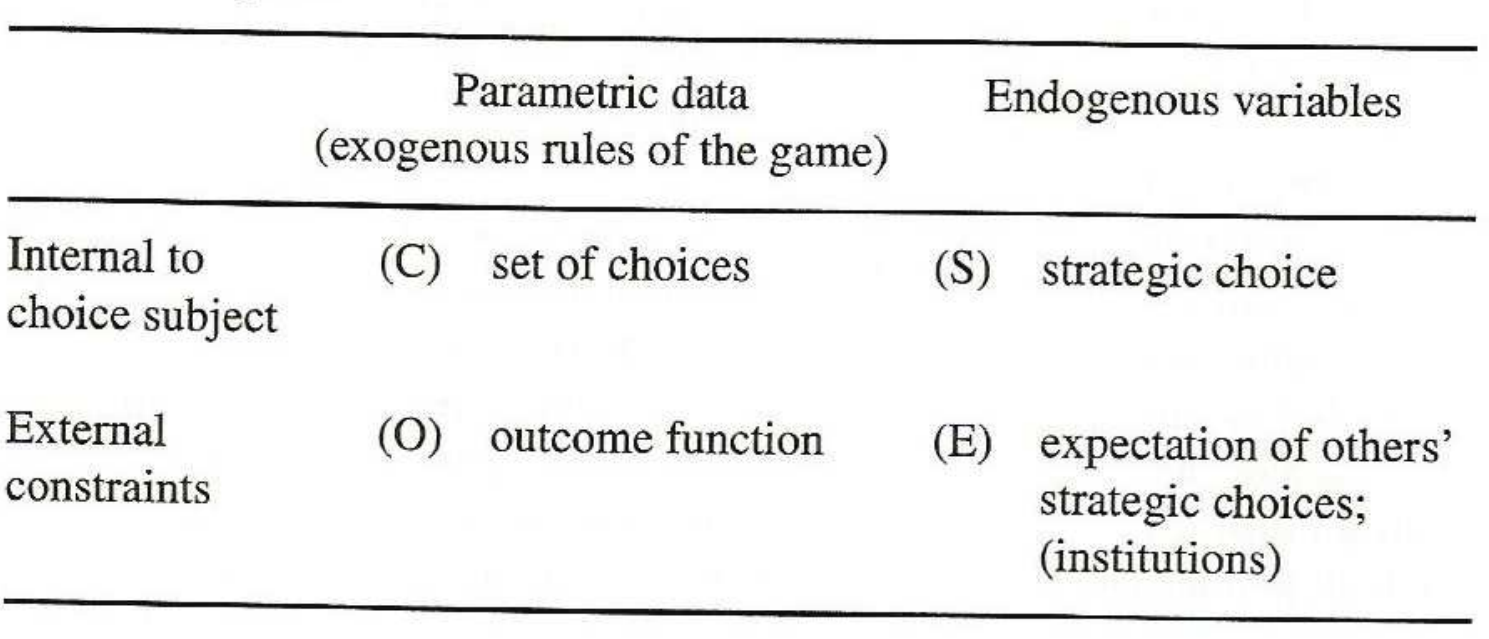
\includegraphics[width=\linewidth]{screenshot001}
\end{figure}


Em seguida, pontua: se as instituições estão associadas a um estado de equilíbrio, qual seria o \textbf{mecanismo de mudança}? Seguindo a perspectiva proposta pelo autor, uma mudança instituição seria a mudança de um equilíbrio para outro associado a uma mudança \textbf{sistemática das estratégias dos agentes}, assim como a representação das percepções dos agentes acerca das instituições.

Nesta abordagem, portanto, a introdução de uma nova lei ou agência regulatória não é nada mais do que uma mudança nas variáveis exógenas na perspectiva do agente. Tal mudança pode provocar um processo de alteração institucional ao criar um ponto focal para que os agentes possam \textbf{alterar suas estratégias} ou por alterar os \textbf{resultados} de suas escolhas. Logo, uma mudança impositiva (``planejada''), pode \textbf{induzir} uma mudança institucional. 

Adiante, o autor questiona: como um agente identifica um momento de mudança estratégica? Após responder em termos da caixa COSE, afirma que quando um agente adota uma regra repetidamente sob as mesmas instituições, esta estratégia é dita \textbf{reprodutível}. Na presença de uma instituição em mudança, o agente adota diferentes regras que considera apropriadas dada estas circunstâncias e desenvolve uma ``meta-regra'' que é acionada sob cada tipo de cenário. No entanto, quando este conjunto de regras é seguindo mediante um conjunto de cenários, este jogo subjetivo é reprodutível. Quando esse conjunto de regras \textbf{não} gera resultados satisfatórios, o agente começa a revisar tais regras mais sistematicamente, gerando \textbf{novas estratégias}, ampliando o conjunto de estratégias existentes. Dito isso, o autor pontua mudanças de estado que podem gerar tais mudanças:

\begin{itemize}
	\item Externos
	\begin{itemize}
		\item Inovação tecnológica permite que outras regras sejam adotadas
		\item Choques externos
		\item $ldots$
	\end{itemize}
	\item Internos
	\begin{itemize}
		\item Experimentos como novas estratégias que não seguem as convenções de um grupo
		\item Jogos repetitivos geram a redistribuição de ativos/poderes, etc
		\item $ldots$
	\end{itemize}
\end{itemize}
Em seguida, o autor argumenta que os choques externos são \textbf{insuficientes} para provocar uma mudanças institucional. Dito de outro modo, na ausência desses fatores endógenos, os agentes podem se adaptar sem que, para isso, seja necessário alterar sua estratégia sistematicamente. Neste ponto, cabe a seguinte passagem sobre mudanças institucionais (p.~27):

\begin{quotation}
	\textit{Once simultaneous revision (innovation) by many agents of their activated
	choice sets and the systemic implementation of new choices therefrom starts,
	the hitherto existing institution will also cease to provide a useful guide/
	constraint for individual choices, because it is no longer an effective summary
	representation of newly emergent choice profiles that can reduce uncertainty in
	agents' expectations. The `taken for granted' premises implied by the institution \textbf{become questionable}. Agents now need to \textbf{process a larger amount of information} regarding the internal state of the domain than they did under the
	rules of the old institution.} 
\end{quotation}

\begin{figure}[H]
	\centering
	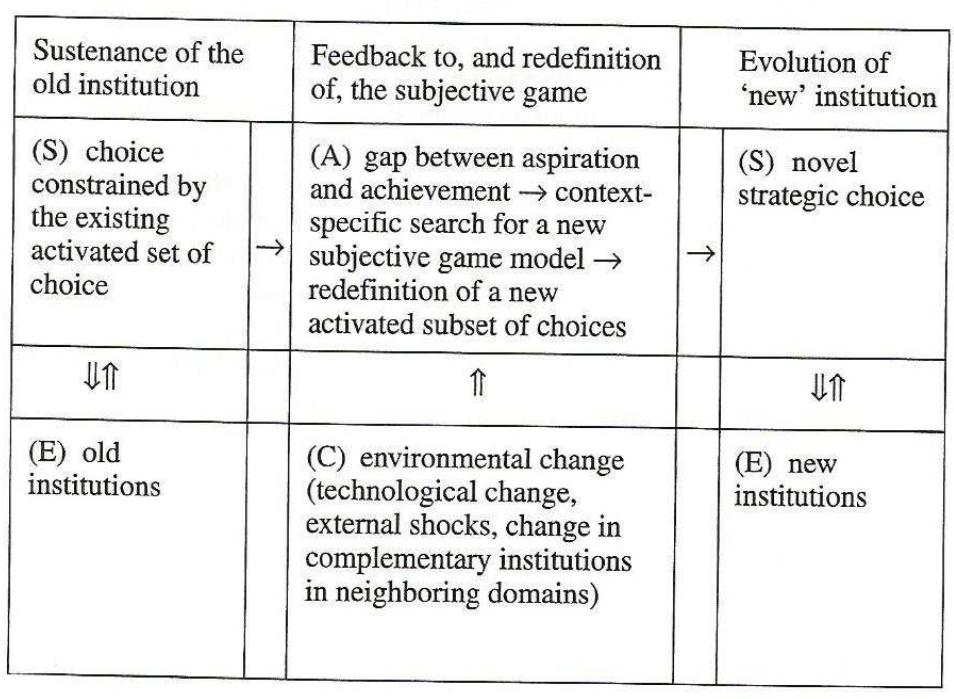
\includegraphics[width=\linewidth]{screenshot002}
	\caption[Mecanismo da evolução institucional]{}
	\caption{}
	\label{fig:screenshot002}
\end{figure}


Um novo equilíbrio deste jogo subjetivo irá se estabelecer quando
\begin{itemize}
	\item A adoção de novas regras não geram uma grande surpresa
	\item O resultado dessa nova estratégia é satisfatório
	\item Haverá uma nova forma de reunir as características subjetivas de um novo perfil de estratégias
\end{itemize}

\section{Conclusões}

O autor identifica alguns mecanismos que são relevantes para a seleção de uma inovação e determinação de suas consequências:
\begin{description}
	\item[Sobreposição dos domínios] As informações do domínio atual mudam ao longo do tempo, mas sua velocidade depende dos tipos de domínio. A avaliação se um mecanismo de mudança institucional é satisfatório só pode ser feito quando se considera o \textbf{contexto histórico}.
	\item[Reconfiguração de padrões] Uma inovação institucional pode emergir como resultado de uma nova ligação entre os domínios
	\item[Complementariedade institucional diacrônica] Uma nova escolha pode não ser viável de forma independente, mas se uma instituição complementar existir, outro domínio ou consolidação entre ambas poderá induzir a criação de novas instituições
\end{description}
Em conjunto, estes mecanismos dão uma característica de \textit{path-dependence} da evolução institucional, bem como uma inovação e subsequente bifurcação. No entanto, para compreendê-los, é preciso de um novo aparato teórico que vá além da teoria dos jogos e que inclua uma comparação histórica.

\end{document}